% =============================================================================
% COPYRIGHT AND DISCLAIMER
% =============================================================================
% This file is provided as a convenience template for competition participants.
% By using it, you accept full responsibility for compliance with all applicable
% copyright, licensing, and usage rules of the Association for Computing
% Machinery (ACM) and of any LaTeX packages you load (including, without
% limitation, the "acmart" document class and related ACM materials).
%
% Consult ACM's official publication, template, and copyright policies before
% using this setup for any purpose other than this competition. Do not assume
% that this template may be reused, redistributed, or submitted elsewhere
% without independently verifying ACM's current rules.
%
% Use of the "acmart" class, the "sigconf" option, or ACM-style formatting in
% this template does NOT mean that this report, this competition, its organizers,
% or any resulting PDF is sponsored, endorsed, affiliated with, or published by
% ACM. ACM trademarks and branding remain the property of ACM.
%
% Template packages live in preamble.tex.
% Citations live in main.bib. Edit this file with your paper content.
% =============================================================================

\documentclass[sigconf]{acmart}
% =============================================================================
% Template setup — participants normally do not edit this file.
% Author content belongs in main.tex; citations belong in main.bib.
% \documentclass lives in main.tex so Overleaf does not treat this file as root.
% =============================================================================

% --- Competition / non-ACM-submission friendly rights metadata -------------
\setcopyright{none}
\settopmatter{printacmref=false}
\acmConference[Kaggle Competition]{Filament Segmentation Challenge}{2026}{\href{https://www.kaggle.com/competitions/filament-segmentation-2026}{kaggle.com/competitions/filament-segmentation-2026}}
\acmBooktitle{Competition Report}
\acmDOI{}
\acmISBN{}

% --- Author guidance text --------------------------------------------------
% \guide{...} is gray italic while \guideStyletrue; omitted from the PDF if false.
% Flip the switch in main.tex after % =============================================================================
% Template setup — participants normally do not edit this file.
% Author content belongs in main.tex; citations belong in main.bib.
% \documentclass lives in main.tex so Overleaf does not treat this file as root.
% =============================================================================

% --- Competition / non-ACM-submission friendly rights metadata -------------
\setcopyright{none}
\settopmatter{printacmref=false}
\acmConference[Kaggle Competition]{Filament Segmentation Challenge}{2026}{\href{https://www.kaggle.com/competitions/filament-segmentation-2026}{kaggle.com/competitions/filament-segmentation-2026}}
\acmBooktitle{Competition Report}
\acmDOI{}
\acmISBN{}

% --- Author guidance text --------------------------------------------------
% \guide{...} is gray italic while \guideStyletrue; omitted from the PDF if false.
% Flip the switch in main.tex after % =============================================================================
% Template setup — participants normally do not edit this file.
% Author content belongs in main.tex; citations belong in main.bib.
% \documentclass lives in main.tex so Overleaf does not treat this file as root.
% =============================================================================

% --- Competition / non-ACM-submission friendly rights metadata -------------
\setcopyright{none}
\settopmatter{printacmref=false}
\acmConference[Kaggle Competition]{Filament Segmentation Challenge}{2026}{\href{https://www.kaggle.com/competitions/filament-segmentation-2026}{kaggle.com/competitions/filament-segmentation-2026}}
\acmBooktitle{Competition Report}
\acmDOI{}
\acmISBN{}

% --- Author guidance text --------------------------------------------------
% \guide{...} is gray italic while \guideStyletrue; omitted from the PDF if false.
% Flip the switch in main.tex after \input{preamble}.
%
% Do not use \guide{...} for \email{...}.
\usepackage{xcolor}
\newif\ifguideStyle
\guideStyletrue
\newcommand{\guide}[1]{%
  \ifguideStyle
    {\color{gray!65}\itshape #1}%
  \fi
}

% --- Math ------------------------------------------------------------------
% Do NOT load amssymb (or amsfonts): acmart already loads newtxmath, which
% defines the same symbols (e.g. \Bbbk) and causes a conflict on Overleaf.
% amsmath is already provided by acmart; mathtools extends it.
\usepackage{mathtools}

% --- Figures ---------------------------------------------------------------
% graphicx is already loaded by acmart
\usepackage{subcaption}

% --- Tables ----------------------------------------------------------------
% booktabs is already loaded by acmart
\usepackage{tabularx}
\usepackage{multirow}

% --- Bibliography style is set in main.tex (ACM-Reference-Format) ----------
.
%
% Do not use \guide{...} for \email{...}.
\usepackage{xcolor}
\newif\ifguideStyle
\guideStyletrue
\newcommand{\guide}[1]{%
  \ifguideStyle
    {\color{gray!65}\itshape #1}%
  \fi
}

% --- Math ------------------------------------------------------------------
% Do NOT load amssymb (or amsfonts): acmart already loads newtxmath, which
% defines the same symbols (e.g. \Bbbk) and causes a conflict on Overleaf.
% amsmath is already provided by acmart; mathtools extends it.
\usepackage{mathtools}

% --- Figures ---------------------------------------------------------------
% graphicx is already loaded by acmart
\usepackage{subcaption}

% --- Tables ----------------------------------------------------------------
% booktabs is already loaded by acmart
\usepackage{tabularx}
\usepackage{multirow}

% --- Bibliography style is set in main.tex (ACM-Reference-Format) ----------
.
%
% Do not use \guide{...} for \email{...}.
\usepackage{xcolor}
\newif\ifguideStyle
\guideStyletrue
\newcommand{\guide}[1]{%
  \ifguideStyle
    {\color{gray!65}\itshape #1}%
  \fi
}

% --- Math ------------------------------------------------------------------
% Do NOT load amssymb (or amsfonts): acmart already loads newtxmath, which
% defines the same symbols (e.g. \Bbbk) and causes a conflict on Overleaf.
% amsmath is already provided by acmart; mathtools extends it.
\usepackage{mathtools}

% --- Figures ---------------------------------------------------------------
% graphicx is already loaded by acmart
\usepackage{subcaption}

% --- Tables ----------------------------------------------------------------
% booktabs is already loaded by acmart
\usepackage{tabularx}
\usepackage{multirow}

% --- Bibliography style is set in main.tex (ACM-Reference-Format) ----------

\usepackage{tikz}\usetikzlibrary{positioning}

% Guide styling: \guideStyletrue = show gray italic hints; \guideStylefalse = omit them
% \guideStyletrue
\guideStylefalse

\begin{document}

\title{Ensemble U-Nets with Soft Annotator Targets and Learned Instance Rescoring}  % Replace this with your title
\subtitle{A Solution to the Solar Filament Segmentation Challenge 2026} % DO NOT CHANGE


\author{Jemin Morabiya}
\affiliation{%
  \country{India}
}
\email{jeminmorabiyawork@gmail.com}

% \author{\guide{Second Author}}
% \affiliation{%
%   \institution{\guide{Your Institution}}  % <- Optional (remove if you are not currently affiliated with any institute)
%   \city{\guide{City}}
%   \country{\guide{Country}}
% }
% \email{second.author@example.com}  % <- Replace with your own email

\begin{abstract}
    This report describes our solution to the Solar Filament Segmentation Challenge~2026, a Kaggle competition on automatic segmentation of solar filaments in GONG H-$\alpha$ observations. We train a 15-model ensemble of U-Nets (three encoder/crop recipes $\times$ five date-grouped folds) that predicts a soft annotator-consensus filament mask together with spine and boundary maps. Probabilities are averaged, turned into disjoint instances by hysteresis grouping, and filtered by a gradient-boosted instance rescorer that estimates each instance's chance of matching an annotator. Under honest 5-fold cross-validation (post-processing and rescorer tuned only on the other folds) the pipeline reaches PQ $0.458\pm0.011$, against $0.33$--$0.35$ for annotator-vs-annotator agreement; the public leaderboard score is $0.39$. Code and weights: \url{https://github.com/jemin-023/filament-seg-2026}.
\end{abstract}

\maketitle

% ==================================== %
%              INTRODUCTION            %
% ==================================== %
\section{Introduction}
    This report goes over the details of our submitted solution to the Solar Filament Segmentation Challenge~2026 \cite{filament-segmentation-2026}. The challenge, launched on July~10,~2026, is organized by the Earth-Space AI Research (ESAIR) Lab\footnote{\href{https://www.esairlab.com/home}{www.esairlab.com/}}. This challenge utilizes the MAGFiLO dataset for evaluation of the segmentation algorithms \cite{ahmadzadeh2024dataset}. The metric is Panoptic Quality (PQ = SQ$\times$RQ) with every annotator of an image scored as a separate ground-truth entry. We measured the human ceiling on the training set: two annotators of the same image reach only PQ $\approx0.35$ (SQ 0.61, RQ 0.55), so label noise dominates and the goal is to predict the \emph{consensus} of annotators rather than any one of them. Our design follows from this: soft targets, ensembling to reduce variance, and post-processing tuned directly on PQ.


% ==================================== %
%              METHODOLOGY             %
% ==================================== %
\section{Methodology}\label{sec:methodology}

\subsection{Data and splits}
We use the 707 unique training images (1154 annotator entries) at full $2048^2$ resolution as single-channel 8-bit input, intensity-normalised. Images from nearby times are nearly identical, so we split by observation date with a stratified group 5-fold (\texttt{StratifiedGroupKFold}, grouped by date, stratified by instrument); all annotators of an image stay in the same fold. Each of the five folds is held out once, giving out-of-fold (OOF) predictions for all 707 images, which we use to tune and honestly evaluate everything downstream.

\subsection{Targets and model}
For every image we average its annotators into three soft targets (Fig.~\ref{fig:pipe}): (0) the filament mask (so annotator disagreement becomes a probability), (1) a spine heat-map (5\,px centreline, Gaussian $\sigma{=}2$) and (2) a thin inner-boundary band. The network is a U-Net \cite{ronneberger2015unet} with scSE decoder attention from \texttt{segmentation\_models\_pytorch}, a 1-channel ImageNet-pretrained encoder and 3 output channels. The loss is BCE+soft-Dice on the mask, plus auxiliary spine (BCE+Dice, weight 0.5) and boundary (BCE, weight 0.3) terms; the auxiliary heads encourage thin structure (barbs) and instance separation. Training uses AdamW, lr $3\!\times\!10^{-4}$, 30 epochs, EMA weights, flips/90$^\circ$ rotations, scale/rotation affine, brightness/contrast/gamma, blur, noise and JPEG-compression augmentation. Three recipes are used, each trained on each of the five folds: EfficientNetV2-S \cite{tan2021efficientnetv2} on 768-px crops, EfficientNetV2-S on 1024-px crops (different seed), and ResNet34 \cite{he2016resnet} on the whole disk downsampled to 1024 px.

\begin{figure*}[t]
\centering
\begin{tikzpicture}[node distance=5mm, every node/.style={font=\footnotesize, align=center},
  box/.style={draw, rounded corners=2pt, minimum height=9mm, inner sep=3pt, fill=gray!8}]
\node[box] (a) {H$\alpha$ image\\$2048^2$, 8-bit};
\node[box, right=of a] (b) {15 U-Nets\\(3 recipes $\times$ 5 folds)\\+ flip TTA};
\node[box, right=of b] (c) {mean probability\\mask / spine / boundary};
\node[box, right=of c] (d) {hysteresis grouping\\$t_{low}$=.15, $t_{high}$=.80\\closing, hole fill};
\node[box, right=of d] (e) {instance rescorer\\(GBM, keep if $p\ge0.35$)};
\node[box, right=of e] (f) {disjoint masks\\$\to$ COCO RLE};
\foreach \x/\y in {a/b,b/c,c/d,d/e,e/f} \draw[->] (\x) -- (\y);
\end{tikzpicture}
\caption{End-to-end inference pipeline (no tiling, $\approx$6\,s per image for 15 models with flip TTA on a laptop GPU).}\label{fig:pipe}
\end{figure*}

\subsection{Inference and post-processing}
Each model predicts the full image (crop models run fully convolutionally on the whole $2048^2$ image) with horizontal-flip TTA; logits are averaged over TTA and \emph{probabilities} over models. Instances are built from the mask probability $P$ by hysteresis: pixels with $P>t_{low}$ (after a radius-1 closing) are grouped into 8-connected components; a component is kept only if it contains a pixel $>t_{high}$, and its pixels are those with $P>t_{shape}$; holes are filled and components smaller than 50\,px dropped. Instances are disjoint by construction. The parameters ($t_{low}{=}0.15$, $t_{high}{=}0.8$, $t_{shape}{=}0.45$) were tuned with Optuna directly on PQ over the pooled OOF predictions.

\subsection{Instance rescoring}
PQ rewards keeping a candidate with match probability $p$ and expected IoU $q$ only if $pq>\mathrm{PQ}/2$, so faint false candidates should be removed even when they pass the thresholds. We fit a gradient-boosting classifier on OOF instances (10 features: log area, mean/max/90th-percentile mask and spine probability, elongation, local contrast, radial position on the disk, number of high-confidence pixels) to predict whether an instance matches some annotator at IoU\,$>0.5$, and drop instances with $p<\tau{=}0.35$ ($\tau$ is chosen fold-out-of-fold).

\begin{figure*}[t]
\centering
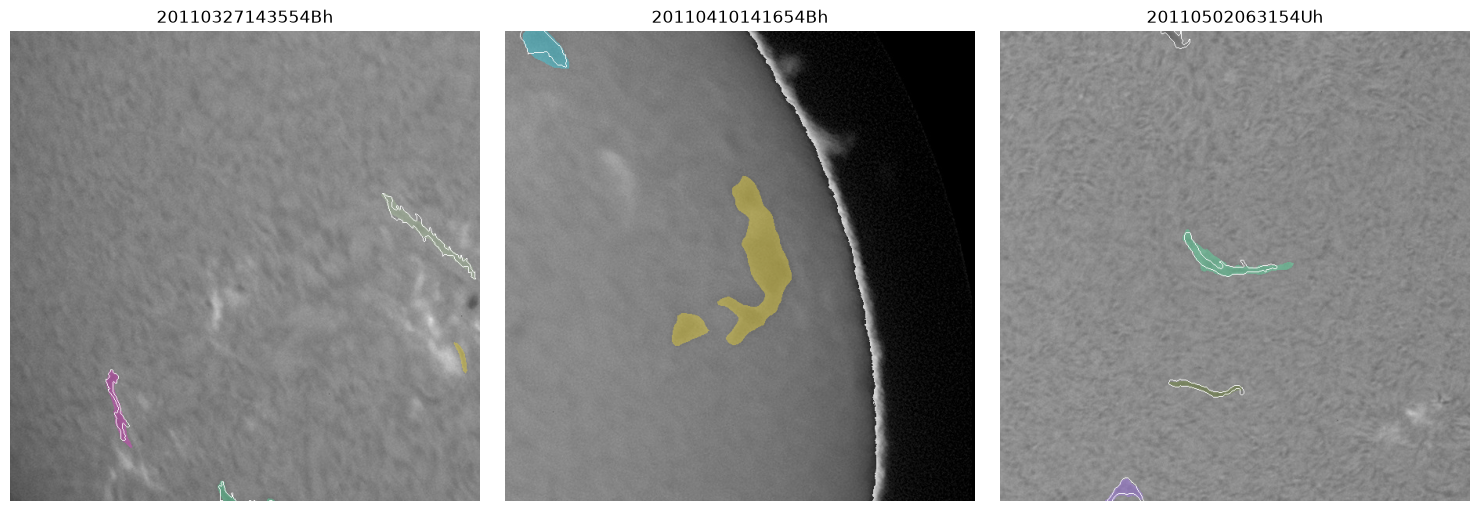
\includegraphics[width=0.88\textwidth]{fig1.png}
\caption{Predictions on held-out fold-0 crops (3 fold-0 models) (coloured = predicted instances, white outline = annotator masks). Predictions follow the annotators' consensus shape; thin barbs and faint fragments remain the main error source.}\label{fig:examples}
\end{figure*}

% ==================================== %
%              EVALUATION              %
% ==================================== %
\section{Evaluation}\label{sec:evaluation}

\subsection{Strategy}
We re-implemented the organizers' scorer (verified: it reproduces the self-evaluation notebook, see \texttt{tests/test\_scorer.py}). All numbers below are \emph{honest}: for each held-out fold, post-processing parameters and rescorer are fit using only OOF predictions of the other four folds, and the models never saw the held-out images. We never tune on the public leaderboard; one submission was used per major model version (v1: 0.38, final: 0.39).

\subsection{Results}
\begin{table}[h]
\caption{Honest cross-validated PQ (mean over folds, std over folds in the last row; 2-fold rows use folds 0--1 only).}\label{tab:res}
\small
\begin{tabular}{lcc}
\toprule
Model & folds & PQ \\
\midrule
ResNet34 (full image) & 0--1 & 0.431 \\
EffNetV2-S, 768 crops & 0--1 & 0.446 \\
Ensemble EffV2S + R34 (10 models) & 0--4 & 0.452 \\
\textbf{Final: 3 recipes, 15 models} & 0--4 & \textbf{0.458 $\pm$ 0.011} \\
\midrule
Annotator vs.\ annotator & -- & 0.33--0.35 \\
Public leaderboard (final) & -- & 0.39 \\
\bottomrule
\end{tabular}
\end{table}
Per fold the final ensemble scores 0.459 / 0.475 / 0.459 / 0.444 / 0.452. The 1024-crop EfficientNetV2-S recipe beat the 768-crop one on all five folds ($+0.004$ to $+0.015$ raw PQ), and adding it lifted the ensemble from 0.452 to 0.458. The rescorer adds $+0.014$ to $+0.021$ PQ when $\tau$ is chosen fold-out-of-fold, but is neutral or slightly harmful when $\tau$ is chosen on a single training fold, so it must be evaluated honestly. A heavy Optuna search (40 trials) over-fitted on small tuning sets; light tuning transferred better. For fold~0 (3 models, 141 images) the model scores PQ 0.472 (SQ 0.69, RQ 0.69) versus 0.333 for annotator-vs-annotator on the same multi-annotated images (Fig.~\ref{fig:examples}).

\subsection{Strengths, weaknesses, improvements}
\emph{Strengths:} the soft consensus targets and ensemble give stable predictions near the annotator-agreement ceiling; the method needs no tiling and runs end-to-end in a notebook with committed weights. \emph{Weaknesses:} (i) the local-to-leaderboard gap ($0.458\to0.39$), which is consistent with sparser test annotations; (ii) one-to-many / many-to-one errors on long filaments (318/221 on pooled OOF), since grouping is threshold-based rather than learned; (iii) small barbs are under-segmented (predicted area $\approx0.8\times$ GT). \emph{Improvements:} learned instance grouping (e.g.\ from the boundary/spine heads), per-observatory calibration, and training the rescorer on more diverse OOF ensembles.

% ==================================== %
%            ACKNOWLEDGMENT            %
% ==================================== %
\section{Acknowledgment}\label{sec:acknowledgment}
    % Do not change
    The organization of the Filament Segmentation Challenge 2026 is partially supported by the U.S. National Science Foundation (NSF) under Grant No. 2209912 and 2433781, directorate for Computer and Information Science and Engineering (CSE), and Office of Advanced Cyberinfrastructure (OAC), and Grant No. 2511630, AST Division Of Astronomical Sciences and MPS Directorate for Mathematical and Physical Sciences.

    The Filament Segmentation Challenge 2026 is sponsored by the U.S. National Science Foundation (NSF) National Solar Observatory (NSO). 

    This work utilizes GONG data obtained by the NSO Integrated Synoptic Program, managed by the National Solar Observatory, which is operated by the Association of Universities for Research in Astronomy (AURA), Inc. under a cooperative agreement with the National Science Foundation and with contribution from the National Oceanic and Atmospheric Administration. The GONG network of instruments is hosted by the Big Bear Solar Observatory, High Altitude Observatory, Learmonth Solar Observatory, Udaipur Solar Observatory, Instituto de Astrofísica de Canarias, and Cerro Tololo Interamerican Observatory.

\bibliographystyle{ACM-Reference-Format}
\bibliography{main}

\end{document}
